\documentclass{kybernetika}
%the class kybernetika includes these packages:
% graphicx, amssymb, amsmath

%DEBUG ONLY
\usepackage{layouts}

%--------------------------------------------------------------------------------------------------
% used environment for theorems:

\newtheorem{theorem}{Theorem}[section]
\newtheorem{lemma}[theorem]{Lemma}
\newtheorem{proposition}[theorem]{Proposition}
\newtheorem{corollary}[theorem]{Corollary}
\newtheorem{remark}[theorem]{Remark}
\newtheorem{fact}[theorem]{Fact}
\newtheorem{example}[theorem]{Example}
\newtheorem{definition}[theorem]{Definition}
\newtheorem{observation}[theorem]{Observation}

\begin{document}

%==================================================================================================
% TITLE PAGE 
%==================================================================================================
\pagestyle{myheadings}
\title{Application of Long Short Term Memory neural networks for GPS satellite clock 
bias prediction}

\author{Piotr Gny\'{s}, Pawe\l{} Przestrzelski}

\contact{Piotr}{Gny\'{s}}
{Department of Computer Science,  Polish-Japanese Academy of Information Technology,
Koszykowa 86 Street, 02-008 Warsaw}{pgnys@pjwstk.edu.pl}

\contact{Pawe\l{}}{Przestrzelski}
{Department of Computer Science,  Polish-Japanese Academy of Information Technology,
Koszykowa 86 Street, 02-008 Warsaw}{pprzestrzelski@pjwstk.edu.pl}

\markboth{Piotr Gny\'{s}, Pawe\l{} Przestrzelski}{LSTM networks for GPS clock bias prediction}

\maketitle

\begin{abstract}
Satellite based localisation systems like GPS or Galileo are one of most commonly used tools
in outdoors navigation. While for most application, like car navigation or hiking, level of
precision provided by commercial solutions is satisfactory it is not always a case for mobile
robots. In case of long time autonomy and robots that operate in remote areas battery usage
and access to synchronization data becomes a problem. In this paper a solution providing a 
real-time on-board clock synchronization is presented. Results achieved are better than current
state of the art solution in real time clock bias prediction for most satellites.
\end{abstract}

\keywords{LSTM, Long Short Term Memory, Neural Networks, GPS, Navigation, Time series prediction}

\classification{68T05, 68T10, 68T40}


%==================================================================================================
\section{Introduction}
Aim of research presented in this paper is do develop an algorithm that will predict bias of
GPS satellites on board atomic clock ensembles bias. Algorithm must be applicable in an 
environment with low computation power available and where battery charge is a highly limited
resource.

%--------------------------------------------------------------------------------------------------
\subsection{Motivation}
During development of an autonomic marine agent one of problems that had to be solved was 
precise navigation. As robot task is to measure quality of water in lakes and small streams
it is expected that it will operate for long time periods in regions where services like 
cellular network may not be available. Additionally a future plans are to develop a model that
will be able to operate on open sea and navigation issues that robots face in such conditions
are even more restrictive on algorithms. With that said main localization technique implemented
will be Global Positioning System which in turn bought issue of limited precision of civilian
variant of GPS as well as it requirement for synchronization with time reference.
For that reason it was decided that there is a need for a on board clock bias prediction to limit
requirement for synchronization.

%--------------------------------------------------------------------------------------------------
\subsection{Contribution}
In following paper a new approach for GPS clock bias prediction based on a Long Short Term Memory
neural networks is presented. For 20 out of 29 satellites that were analysed in this work 
prediction results were better than current state of the art and for 6 of them results were
significantly better. Results of presented research can be used in a offline GPS receiver as 
a alternative for IGU provided products.


%==================================================================================================
\section{Clock bias in GNSS}
Due to the nature of GNSS precision time measurement is crucial for accurate localisation.
In this section information a basic explanation of how GNSS services work will be presented
as well as more in depth description of clock ensemble implementation and bias modeling.
Current state of the art will be presented as well however no details about underlying 
mathematical model will be shared as this is beyond scope of this paper.

r---------------------------------------------------------------------------------------------------
\subsection{Importance of clock bias in localisation}
All global satellite navigation systems (GNSS) are variant of beacon based localization
systems\cite{Blewitt1997}.Such systems require information about beacon position
and distance between localized object and beacons.
With that information it is possible to calculate position of object in same reference
frame as that of beacons.
Both of those tasks are much more difficult in GNSS due to a nature of the beacons.
Unlike in case of a stationary beacons GNSS satellites move with high speed so
their position must be calculated based on satellite ephemeris\cite{Vallado2008}.
Another problem is distance measurement which without specialised equipment must be
done with time of arrival (ToA) instead of angle of arrival (AoA) or
received signal strength (RSS) \cite{Doberstein2012}.
When measuring distance by ToA  3 properties of a signal must be known:
\begin{itemize}
\item $t_o$ : time of origination
\item $t_a$ time of arrival
\item $v$ velocity
\end{itemize}
In case of GNSS system signal is a electromagnetic wave therefore its speed is equal
to speed of light $c\approx 3*10^{9} \frac{m}{s}$. Time of arrival is recoded when
data frame wave front reaches receiver, this means that receiver time is used.
Origination time is recorded on satellite according to it local clock and
included in data frame. Thanks to that distance can be calculated by following 
equation:
\begin{equation}
  d=c*(t_a-t_o)
\end{equation}
However $t_a$ and $t_o$ are using different reference frames so for comparison
to be possible they must be transformed into a common reference frame.
This is referred to as a synchronisation of the clocks and is very important as
a de synchronisation on level of single nanosecond results in about 30 cm of
positioning error\cite{Enge2011}.
While actual calculations 

%--------------------------------------------------------------------------------------------------
\subsection{IGU products}
The most widely used source of precise clock corrections are products provided 
by International GNSS Service (IGS) \cite{IGS}.
\begin{table}[ht] 
	\centering
	\caption{Variants of IGS products}
	\label{tab:igs_products}
	\begin{tabular*}{\textwidth}{*{5}{l}}
		\hline
		\hline
		Type& Accuracy& Latency& Update& Sample \\
		&&&&interval\\
		\hline
		Broadcaster & 5ns & real time & -- & daily  \\
		Ultra rapid -- predicted & 3ns & real time & at 03, 09, 15, 21 UTC & 15 min  \\
		Ultra rapid -- observed & 150ps & 3-9 hours & at 03, 09, 15, 21 UTC & 15 min  \\
		Rapid & 75ps & 17-41 hours & at 17 UTC daily & 5 min \\
		Final & 75ps & 12-18 days & every Thursday & 30 s \\
		\hline
		\hline
	\end{tabular*}
\end{table}
Values shown in Table \ref{tab:igs_products} refer to satellite clock bias only,  IGS products
provide other information which full description  is available at online repository. 
IGS products can be easily divided into two categories:
\begin{itemize}
	\item real time consisting of transmitted and ultra rapid predicted half,
	\item high latency consisting of ultra rapid observed half as well as rapid and final products.
\end{itemize}
Solutions that have high latency are not usable in real-time navigation and as such will not be
considered in this work. Ultra-rapid observed part will be used as a source of
reference time so that if a bias prediction error is equal to zero it means that is
the same as provided by Ultra-rapid observed.
As can be seen in the Table \ref{tab:igs_products} all real-time solutions provide precision 
at a range of nanoseconds, aim of this work is to show that LSTM networks can provide 
better results than those solutions while still working at real-time response latency.

%--------------------------------------------------------------------------------------------------
\subsection{Data source}
This work focuses only on GPS satellites which are divided into five groups :
Original (II), IIA, ,IIR ,IIR-M ,IIF.
As original generation was full retired in 2007 it will not be taken into consideration, while
a single satellite from generation IIA was used in second phase of experiments it was no longer
present in following phases as that generation was fully retired in 2019.
This results in 31 individual satellites for phases 1 and 2 and 30 for phases 3 and 4.
Almost all of them are equipped with Rubidium clock ensemble witch exception of two satellites
from generation IIF that use Cesium clocks instead.
Each satellite have an assigned space vehicle number (SVN) and pseudo random noise (PRN).
In this work a PRN will be used as a identifier as it is unique for every active satellite, 
although it can be used again after said satellite gets retired, and ranges from 1 to 32.
\begin{table}[ht] \label{table:2}
\parindent0pt
\caption{Bias prediction error in relation to regularization and dropout level}
\centering
\begin{tabular}{ l  c  c }
  \hline
  \hline
  Generation& clock type& satellites\\  \hline
  IIA & Rb& 18\\  
  IIR & Rb& 2 11 13 14 16 19 20 21 22 23 28\\ 
  IIR-M & Rb& 5 7 12 15 17 29\\ 
  IIF & Rb& 1 3 6 9 10 25 26 27 30 32\\ 
  IIF & Cs& 8 24 \\ \hline \hline
 \end{tabular}
\end{table}
For satellites with rubidium based clock ensembles bias have a very distinct constant drift
that makes data appear linear, it can be seen for satellites 01 and 08. 
On the other hand in case of cesium based clock ensembles for which constant drift is much 
smaller other sources of bias are visible, like seen for satellite 24.
There is also a single satellite for which, during observed period, constant drift was almost
not present. This was satellite 14 and while no official source of information describes this 
behaviour
\begin{figure}[ht] 
\centering
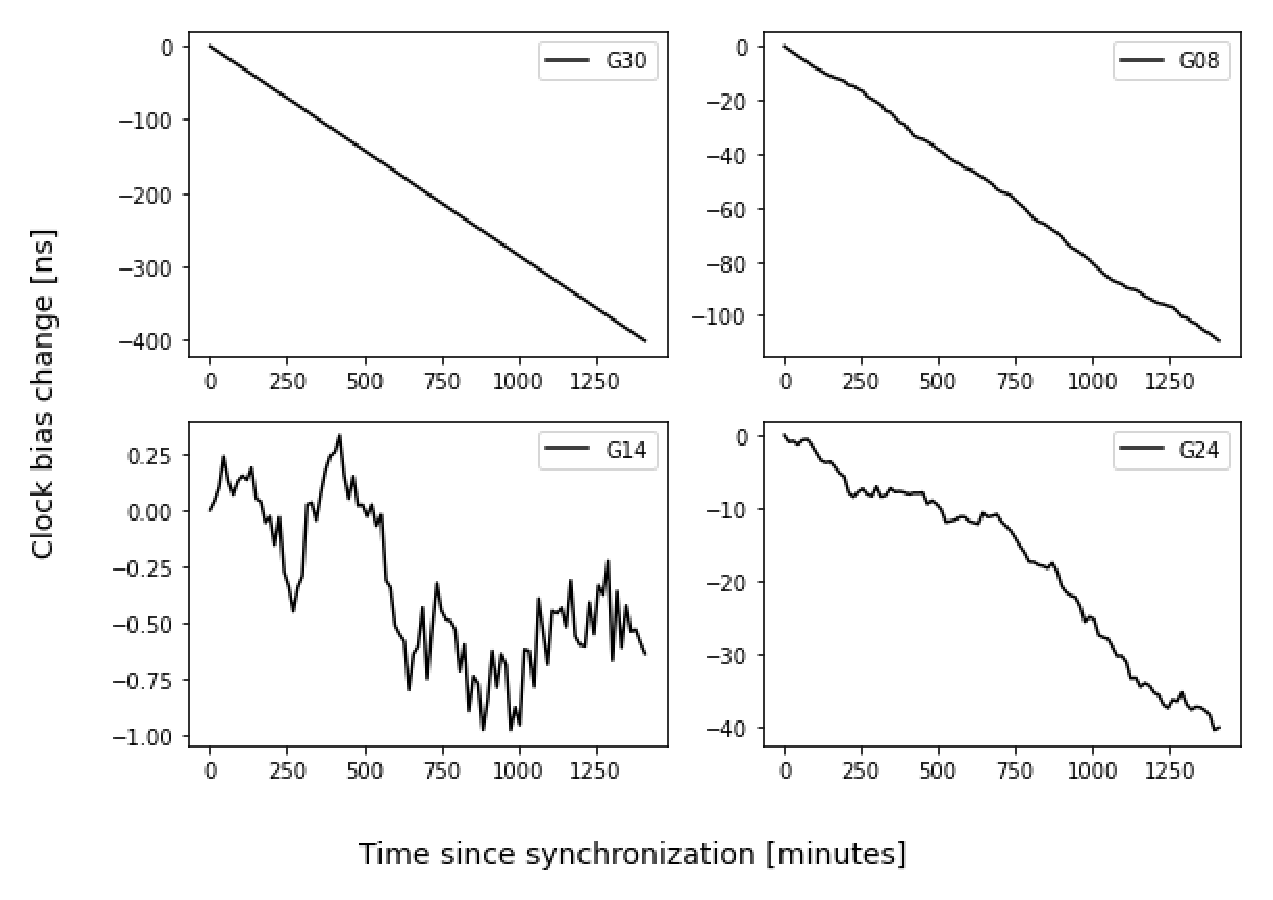
\includegraphics[width=\textwidth]{figures/bias_raw}
\caption{Raw clock bias}
\label{fig:bias_raw}
\end{figure}

%--------------------------------------------------------------------------------------------------
\subsection{Preprocessing}
IGU provides raw clock bias, this poses two problems for approach used in this work.
Firs one is that constant clock drift is such a major source of bias that it overshadows other
sources as seen on figure \ref{fig:raw_bias} in visualisation data seams to be linear.
Second issue is non-stationary nature of series, this is a problem as neural networks work best
fro stationary data with mean at 0 and values in between -1 and 1. To solve those problems firs
series is diffed which returns data where other noises besides constant drift are visible as
seen on figure \ref{fig:diffed_bias}.
\begin{figure}[ht] 
\centering
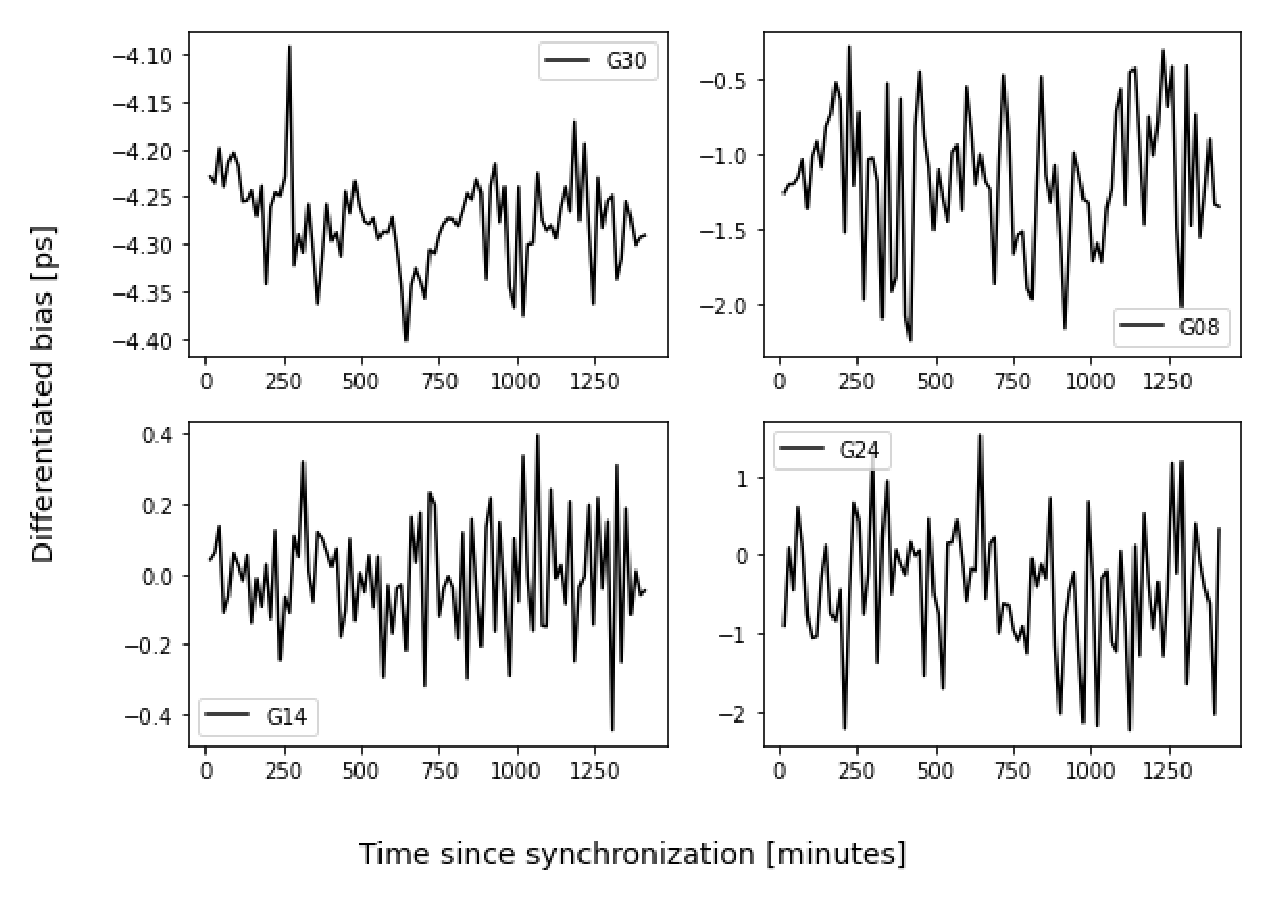
\includegraphics[width=10cm]{figures/bias_diffed}
\caption{Differentiated clock bias}
\label{fig:diffed_bias}
\end{figure}
Constant drift is still present as shift at y axis, to remove it a mean shift must be performed.
Finally data must be scaled so that there will be no values with absolute value above one. It is
of course possible for future prediction inputs to have absolute value above one however this will
not be a problem as network can deal with such inputs especially if they appear rarely in series.
Another issue is whether to use same preprocessing for all satellites or should each of them 
have their own parameters.
Analyse of data shown on figures \ref{fig:diffed_diffs} and \ref{fig:diffed_shifts} shows that
constant shift as well as value range for mean shifted data can vary radically between satellites.
Because of that a separate preprocessing parameters are used for each satellite.

\begin{figure}[ht] 
\centering
	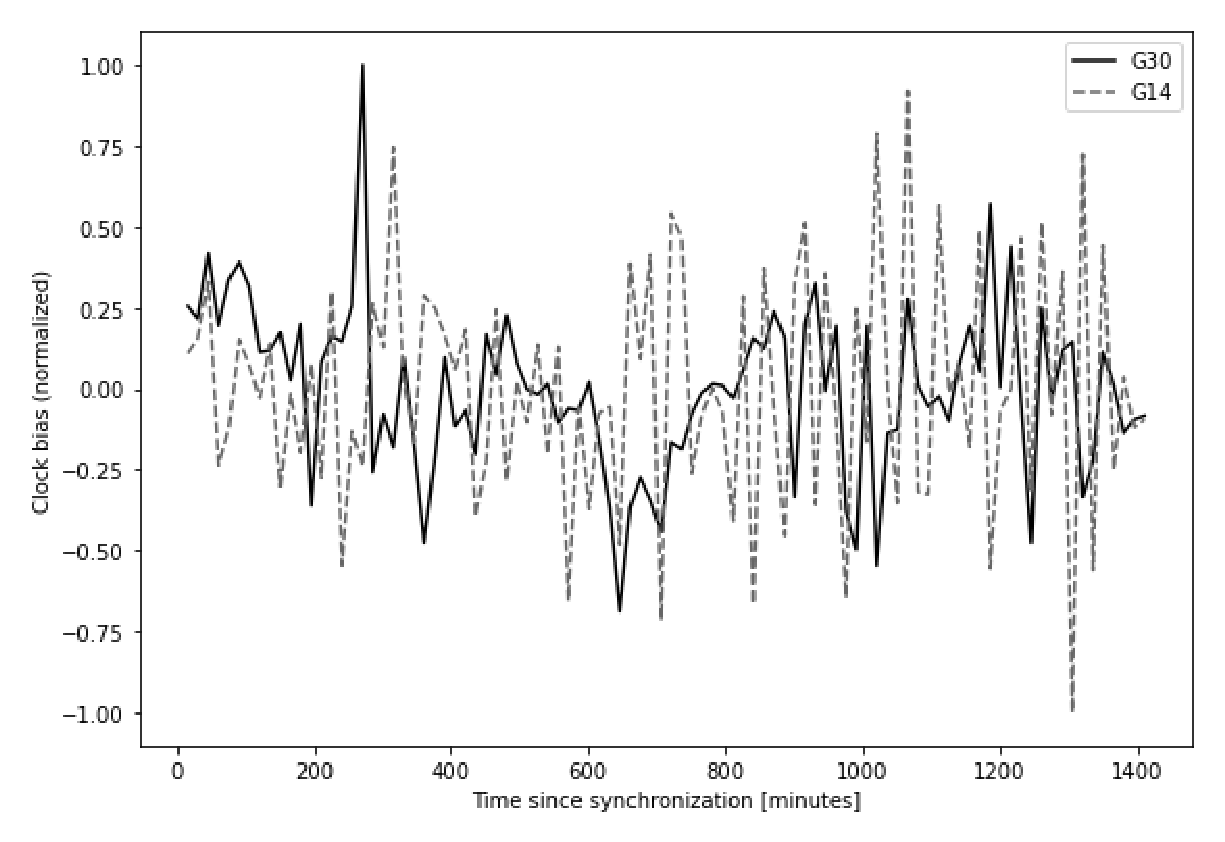
\includegraphics[width=10cm]{figures/bias_normalized}
\caption{Comparison of diffed clock bias}
\label{fig:diffed_shifts}
\end{figure}

%==================================================================================================
\section{Neural networks}
Machine learning (ML) approaches based on a artificial neural networks (ANN) are
well established as a efficient pattern detectors \cite{Abiodun2019} \cite{Miller1993}
\cite{Faraway2008} \cite{Herbrich1999} \cite{Khan2019}.
It has also been used in GNSS systems especially since advent of the deep learning
algorithms \cite{Wei2016} \cite{Kim2019} \cite{OrusPerez2019}.
One of it uses is prediction of clock bias \cite{Wang2017} \cite{Indriyatmoko2008}
which as mentioned in previous section is an essential value in positioning calculations.

%--------------------------------------------------------------------------------------------------
\subsection{Overview}  
Like all digital signal processing applications software neural networks operate in
discreet time and discreet amplitude domain. This is the reason why a time series clock model
was chosen. Basic model of neuron (neural layer) was created by McCullough and Pitts in 1943
\cite{McCulloch1943}. It described response of neural layer to multiple signals with
equation $y= \chi (W*x+b)$ where $y$ is response, $x$ input, $W$ weights and $b$ bias.
Algorithm for automated adjustment of weights in relation to data was proposed in 1958
While this model and its successors where inspired by a biological neuron there are much
more simplified. One of those simplification is lack of time domain in model which means
that response of a layer depends only on its current input.
This is in contrast with biological networks that are sensitive not only for signal value
but also for its change over time.

%--------------------------------------------------------------------------------------------------
\subsection{Long Short Term Memory networks}
Simple solution to problem of time independence is to concatenate response of neural layer
from previous cycle to it input $x'(t)=[x(t)|y(t-1)]$.
Such solution results in signal propagating trough time and influencing responses of future cycles,
if this is only modification to feed forward model such layer is called simple recurrent
unit (SRU).
While this solution makes model time aware it have its own problems, mainly a signal vanishing
issue. Since the input signal from cycle $n$ have direct influence only on a response of this
cycle and for each subsequent cycles it is only trough feedback loop. Influence of input $n$ on
response of cycle $n+k$ grows inverse proportional to $k$.
This means that in this model only those regularities that appear over short time periods can
be detected.
Making weights on feedback bigger will not eliminate problem and instead replace it with signal
explosion that causes response to reach maximum value if a strong signal appeared on input at
least once.
One of possible solutions to this issue is addition of long term memory which will regulate
forward and loop back path influence on neuron response, such solution is used in long short
term memory (LSTM) networks \cite{Hochreiter1997}.
\begin{figure}[ht] 
\centering
	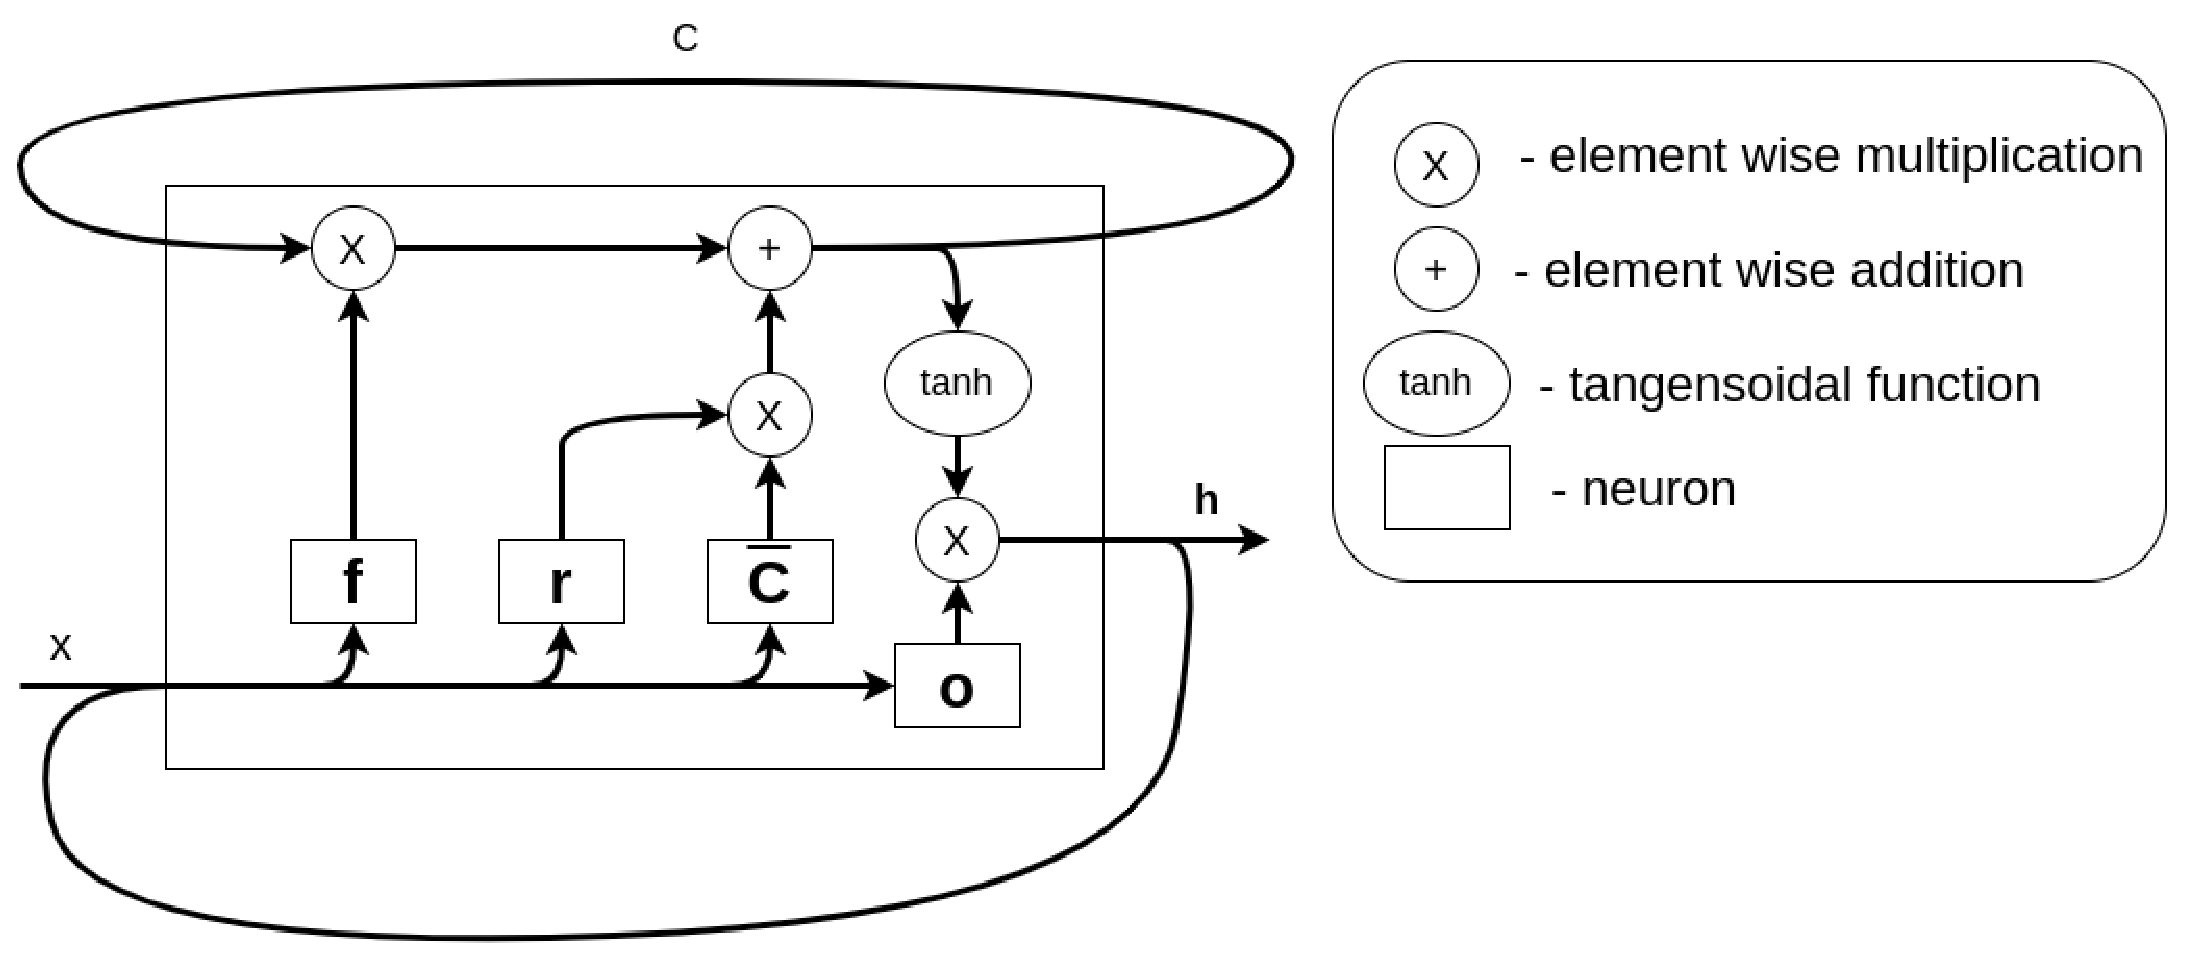
\includegraphics[width=10cm]{figures/lstm}
\caption{LSTM layer}
\label{fig:lstm}
\end{figure}
Single LSTM neuron consists of 4 basic neurons and two non neuron operations:
\begin{itemize}
\item $x'(t)=[x(t)|y(t-1)]$
\item $o_t=\sigma (W_o\cdot x'_t+b_o)$
\item $r_t=\sigma (W_r\cdot x'_t+b_r)$
\item $f_t=\sigma (W_f\cdot x'_t+b_f)$
\item $\bar{C}_t=\tanh (W_c\cdot x'_t+b_c)$
\item $C_t=f_t\circ C_{t-1}+r_t\circ \bar{C}_t$
\item $y_t=o_t\circ \tanh (C_t)$
\end{itemize}
With $W$ and $b$ being weights and biases for each basic neuron, $x$ input, $y$ output and
$C$ long term memory. As it can be seen $o_t$ is a equivalent of SRU and is moderated by
long term memory before propagating as output. Temporary value of long term memory based
only on current output $\bar{C}_t$ is calculated and then with help of neurons $r$ and $f$
is transformed into its final value.
Neuron $r$ is called remembering gate and influences to what degree temporary long term
memory from given cycle effects its final value while $f$ is forgetting gate and
decides influence of long term memory from last cycle on current one.
Thanks to such implementation model can learn to detect long term regularities as well
as short term ones.

%--------------------------------------------------------------------------------------------------
\subsection{Overfitting}  
Overfitting takes place when estimator function is adjusted to training data to such high
degree that it can no longer function as a general predictor.
For example if a network that is supposed to recognise cats will be trained on set that contains
only sphinxes it may be unable to classify other breeds as cats.
Overfitted networks provide very high quality results as long as input overlap with test set
otherwise quality of results drop sharply.
In case of satellite clocks predictor can overfitt in regards to following parameters:
\begin{itemize}
\item clock type
\item location (orbit)
\item epoch
\end{itemize}
When selecting a solution a decision must be made on what level of generalisation model should
represent. Limiting predictions to same epochs that were used for training is in contradiction
with network main goal, predicting future biases. However as satellites use different models
of atomic clocks and are placed on different orbit attempts at generalisation for those
proprieties risk to high precision trade off.
Therefore a separate network will be used for each satellite that will be unable to generalize
its predictions to others.

%==================================================================================================
\section{Experiments}
Main aim of experiments was to determine if it is possible for small LSTM network to 
achieve results comparable with IGU rapid predictions that are considered state of the art.
First tests were made on a single satellite and prediction results were compared against 
polynomial regression as well as IGU. As results were already better than IGU for first attempts
any following tests were executed on almost complete set of satellites. This set did not included
those satellites that were activated or retired during experiment period.
%--------------------------------------------------------------------------------------------------
\subsection{Overview}
Experiments were divided in three phases:
\begin{enumerate}
\item In first phase a single satellite was selected and prediction with generic LSTM architecture
	was made. Then it was compared against polynomial regression as well as IGU rapid predictions.
	While achieving results better than polynomial regression would be considered acceptable at 
	this stage would be considered acceptable LSTM proved to be better than IGU example which
	was considered state of the art. Because of that a decision was made not to adjust network
	model at this stage, as was originally intended, but move to next stage with a initial model.

\item In second phase network developed in first phase was tested on set of all active 
	satellites and compared against IGU rapid prediction. At this phase comparison against 
	polynomial regression was dropped as achieving results worse than IGU was no longer 
	considered acceptable. In this phase for 5 of 31 satellites LSTM achieved better 
	results than IGU.

\item As second phase provided acceptable results only for a small group of satellites 
	an alternative architectures were tested, more details about them will be written in 
	dedicated section. In this phase results better than IGU were achieved 
	for 13 of 30 satellites.
\item Final phase was dedicated to tuning learning meta parameters and it results are described
	in more details in section dedicated to experiments.

\end{enumerate}

%--------------------------------------------------------------------------------------------------
\subsection{Comparison with state of the art}
Over the course of experiments a multiple network architectures were tested, in this paper
main focus will be given to experiments from phase 4 where general architecture was already
selected.
Final architecture is a 3 layer network with 2 hidden LSTM layers, first one with size equal
to input and second double that size. Third layer consists of single densely connected neuron
that outputs a single prediction step.

\begin{figure}[ht] 
\centering
	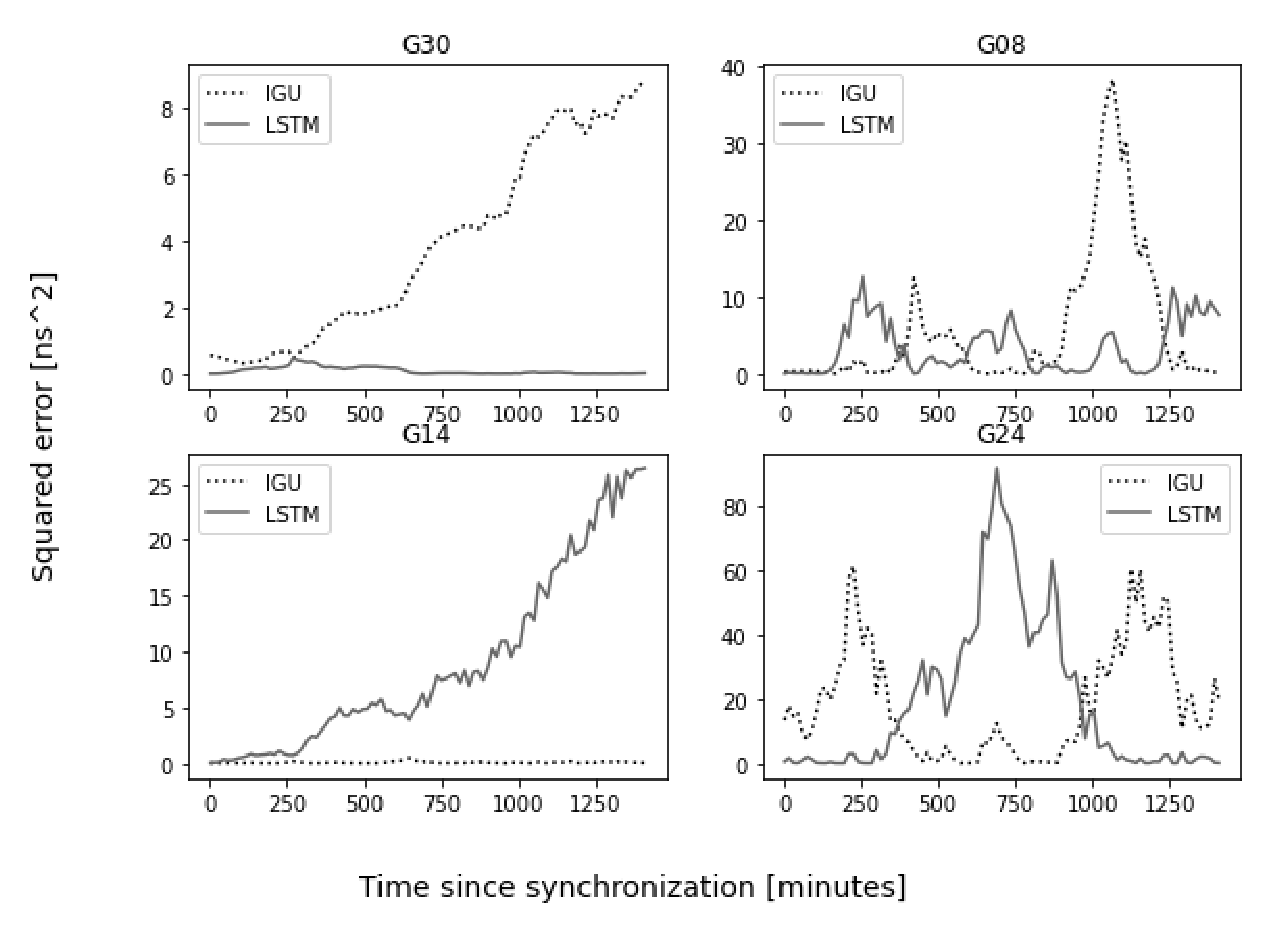
\includegraphics[width=10cm]{figures/error_overwiev}
\caption{Squared error}
\label{fig:error_overview}
\end{figure}
As can be observed on plots presented on Figure \ref{fig:error_ovevwiew} there are satellites
for which results achieved by LSTM network are significantly better than current state of the
art and that difference only deepens with prediction time. Examples of such situation are
satellites G07, G10 or G30. Other group represented by satellites G14, G15 or G17 are those 
for which results of LSTM are clearly worse. Another group consists of satellites for which 
squared error is smaller for initial period of prediction however it rises with time resulting
in predictions worse than IGU. Examples of such behaviour are visible in satellites G01
G09 and G29. Last of groups contains satellites for which prediction quality can vary over
time like in case of G08.
\begin{figure}[ht] 
\centering
	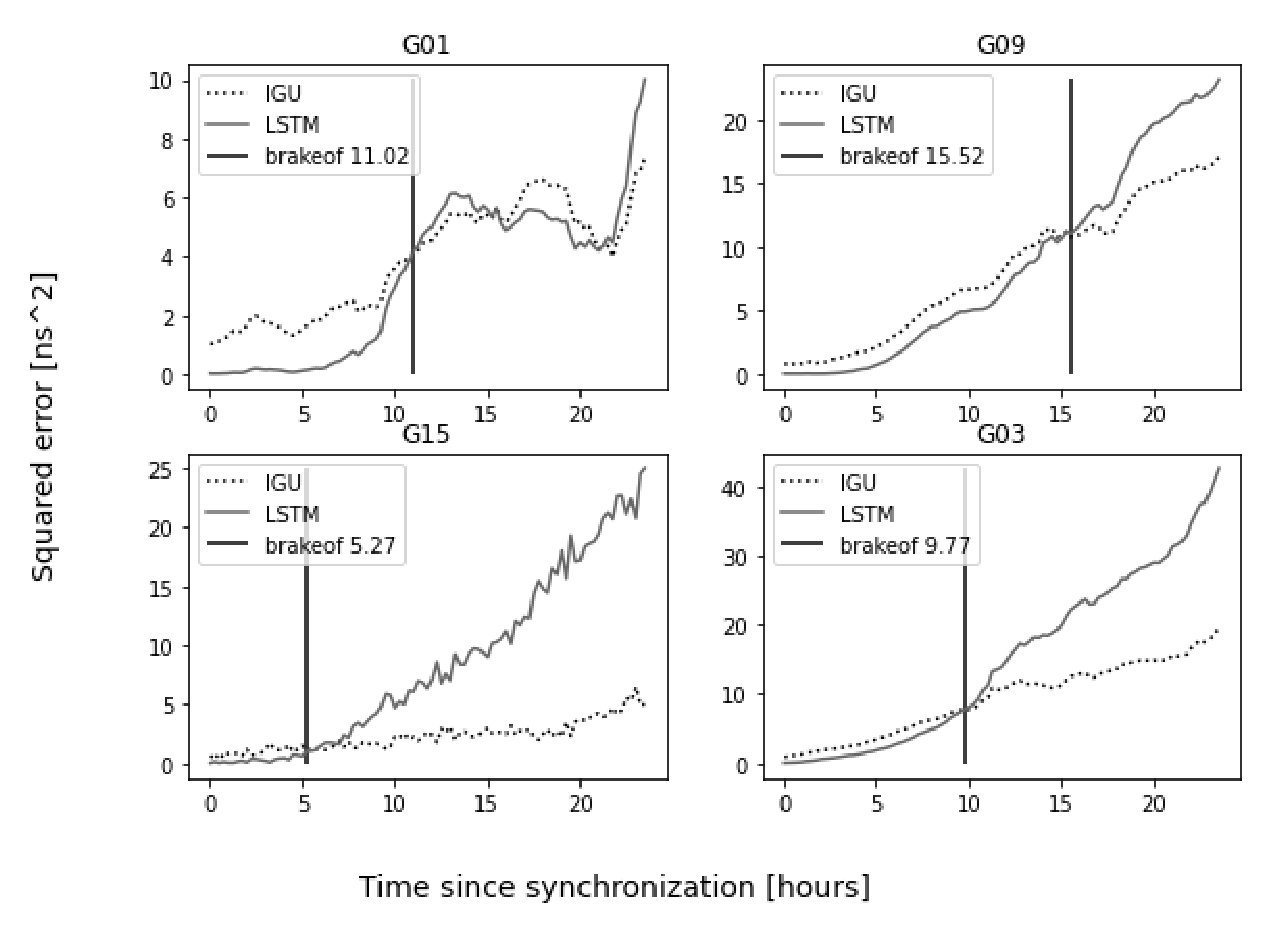
\includegraphics[width=10cm]{figures/brakeoff_compare}
\caption{Comparison between LSTM and IGU predictions}
\label{fig:cutoff}
\end{figure}
As it is shown on Figure \ref{fig:cutoff} in case of some satellites period for which LSTM
have advantage over IGU predicted part is longer than 9 hours. This is important value as 
as after that period a synchronization witch IGU observed product can be made.
IGU observed products have picoseconds level precision which is satisfactory for most 
robotic implementation.

\begin{table}[ht] \label{table:result}
\parindent0pt
\caption{Quality of results }
\centering
\begin{tabular}{ l  c  c }
  \hline
  \hline
  Result category & satellites\\  \hline
  Superior & 07 10 12 19 26 30\\  
  Superior for acceptable time period& 01 03 09 13 23 27 28 29 31\\ 
  Varied & 05 08 24 16\\ \hline \hline
  Superior for short time period& 11 15 \\ 
  Inferior & 02 06 14 17 21 22 25\\ 
 \end{tabular}
\end{table}

As superiority over 9 hour period is enough to consider LSTM solution a preferable one to
IGU rapid prediction for experiments in this paper success was achieved for 68/% 
cases.

%==================================================================================================
\section{Conclusions}
Experiments described in this paper have proven that even relatively simple LSTM network can
handle bias prediction well. That indicates possibility of application of this system in 
low power embedded system which was motivation for this research. Future modification to network
may include addition of new layers or utilization of more data from SP3 files.
However this steps will be made only after network developed in this work will be implemented and
benchmarked on embedded systems ranging from powerful ones like Raspberry Pi down to ones
with very limited processing and memory resources like STM32L series.
\makesubmdate

%==================================================================================================
\bibliography{bibliografia}{}
\bibliographystyle{plain}

\makecontacts

\end{document}


